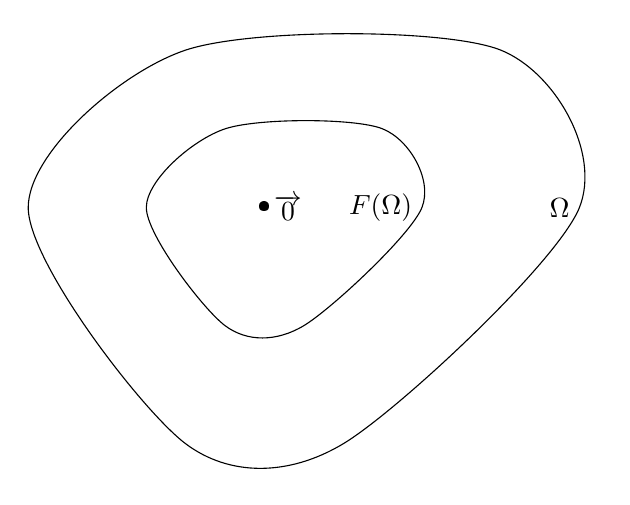
\begin{tikzpicture}


\usetikzlibrary{calc}


\draw plot[smooth cycle]
	coordinates {(-3,0) (-1,-3) (1,-3) (4,0) (3,2) (-1,2)};
	
\draw plot[smooth cycle]
	coordinates {(-3/2,0) (-1/2,-3/2) (1/2,-3/2) (4/2,0) (3/2,2/2) (-1/2,2/2)};
	

\node at (4,0) [left] {$\Omega$};

\node at (2,0) [left] {$F(\Omega)$};

\node at (0,0) [right] {$\overrightarrow{0}$};

\draw (0,0) node {\textbullet}; 

\end{tikzpicture}